%% DO NOT CHANGE THIS PART
\documentclass[graybox,envcountchap,sectrefs]{svmono}
\usepackage{type1cm}         
\usepackage{makeidx}         % allows index generation
\usepackage{graphicx}        % standard LaTeX graphics tool
\usepackage{multicol}        % used for the two-column index
\usepackage[bottom]{footmisc}% places footnotes at page bottom
\usepackage{newtxtext}       % 
\usepackage[varvw]{newtxmath} % selects Times Roman as basic font
\usepackage{caption}
\DeclareCaptionLabelFormat{myfig}{#2. ábra}
\captionsetup[figure]{labelformat={myfig},labelfont=bf}
\DeclareCaptionLabelFormat{mytable}{#2. táblázat}
\captionsetup[table]{labelformat={mytable},labelfont=bf}
\RequirePackage{tikz}
\usepackage[absolute,overlay]{textpos}
% For usage of rotated array with newlines in the cells
\usepackage{array}
\usepackage{makecell}
\renewcommand\theadalign{bc}
\renewcommand\theadfont{\bfseries}
\renewcommand\theadgape{\Gape[4pt]}
\renewcommand\cellgape{\Gape[4pt]}
\usepackage{url}
\usepackage{blindtext, rotating}
\makeindex             % used for the subject index
%%%%%%%%%%%%%%%%%%%%%%%%%%%%%%%%%%%%%%%%%%%%%%%%%%%%%%%

% Data for the title page
\Address{1034 Budapest, Bécsi út 96/b}
\TaxID{123456}
\ContractNumber{UNKP2020-AA-BB-11223344}
\StartDate{2020.09.01.}
\EndDate{2021.08.31.}
\Supervisor{Prof. Dr. Pitagórasz} %empty if you don't have one
\Webpage{www.home.oe} %empty if you don't have one

\author{Rezső Dezső}
\title{\Huge Pitagórasz-tétel PYTHONban}
\subtitle{Életem főműve} %empty if you don't have one

\begin{document}
%UNKP logo on the title page
\begin{textblock*}{0.65\textwidth}(3.659cm,1.72cm)
	
\includegraphics[width=0.7\linewidth]{img/unkp_logo-04}
\end{textblock*}
%BARK logo on the title page, change if you aren't entitled to use it :D
\begin{textblock*}{0.74\textwidth}(9.259cm,2.102cm)
	
\includegraphics[width=\textwidth]{img/OEBARKHUNLEFT.pdf}
\end{textblock*}

\maketitle

%%%%%%%%%%%%%%%%%%%%%%% 

\section{AZ ELÉRT EREDMÉNYEK}

1-1 oldalas RÖVID ÖSSZEFOGLALÓ 

\subsection{A kutatási projekt előzményei és célkitűzései}

A szakaszt a nyilvános közzététel követelményéneknek megfelelő minőségben (nyelvezettel) kell megfogalmazni, úgy, hogy lehetővé tegye az egyetem honlapján történő közvetlen, további szerkesztői munkát nem igénylő közzétételt. Könnyen olvashatónak kell lennie, vagyis a szélesebb nyilvánosság számára is érthető nyelven kell írni, ezáltal elősegítve az ÚNKP által finanszírozott eredmények terjesztését. Hossza – szóközökkel együtt – nem haladhatja meg a 7500 karaktert (amely megfelel egy szöveges dokumentum két oldalának). Ez a szakasz nem tartalmazhat bizalmas adatokat.
A kiadvány összefoglalását „önálló” szövegként kell elkészíteni. Nem kell hivatkozni a kutatás során keletkezett egyéb dokumentumokra, a hivatkozások csak nyilvánosan elérhető információkra vonatkozhatnak.
Az összefoglalóban a projekt munkáját szemléltető diagramok és fényképek szerepelhetnek.
A támogatásból megvalósult program eredményét ki kell emelni a beszámolóban

\subsection{A kutatás eszközei és módszertana}

\subsection{A támogatási időszakban elért legfontosabb eredmények}

\subsection{A projekt újdonságtartalma, a folytatásban várható további eredmények, hatások (beleértve a tágabb, társadalmi-gazdasági hatásokat is) bemutatása}

Tehát az eredmények szöveges összefoglalására összesen 6 oldal áll rendelkezésre. \footnote{Ezt nem értem, hogy jött ki, ha valakinek van sejtése, írja meg... KJ}

\section{AZ EREDMÉNYEK NYILVÁNOSSÁGRA HOZATALA}

\subsection{Tudományos publikációk}

Az alábbi adatok megadása kötelező: publikáció típusa, címe, DOI azonosító (ha van), szerző(k), folyóirat/kiadvány címe, sorszáma, kiadó, kiadás helye, időpontja, oldalszám, referált kiadvány (I/N), open-access kiadvány (I/N)

A saját megoldásom\footnote{KJ} erre, akinek tetszik, használja:

\hspace{2cm}
\begin{turn}{90}
	{\small
		\begin{tabular}{|c|c|c|c|}
			\hline
			Típus: & konferencia & konferencia & folyóirat (D1) \\
			\hline
			Cím: & \makecell{Decreasing the {Computational} \\ {Demand} of {Unscented} {Kalman} \\ {Filter} based {Methods}} & 
			\makecell{Computational {Analysis} of {Relaxed} \\  {Unscented} {Transformation} in  terms of \\ necessary floating point operations} &  
			\makecell{Computationally Relaxed \\ Unscented Kalman Filter} \\
			\hline
			DOI: & 10.1109/SACI51354.2021.9465610 & 10.1109/INES52918.2021.9512926 & - \\
			\hline
			Szerzők: & Kuti J{\'o}zsef, Galambos P{\'e}ter &  Kuti J{\'o}zsef, Galambos P{\'e}ter & \makecell{Kuti József, Rudas Imre,\\ Galambos Péter}  \\
			\hline
			Megjelentető: & \makecell{15th {International} {Symposium} on \\  {Applied} {Computational} {Intelligence} \\ and {Informatics} ({SACI})} & 
			\makecell{25th {International} {Conference}  on\\  {Intelligent} Engineering Systems ({INES})} &
			\makecell{IEEE Transactions \\ on Cybernetics}  \\
			\hline
			Kiadó: & IEEE & IEEE  & IEEE \\
			\hline
			Kiadás helye: & Timisoara, Romania & Budapest, Hungary & New York, USA \\
			\hline
			Időpontja: & 2021 & 2021 &  - \\
			\hline
			Oldalszám: & 181--186  & 55--60 & - \\
			\hline
			Referált kiadvány: & Igen & Igen & Igen \\
			\hline
			Open-access kiadvány: & Nem  & Nem & Nem \\
			\hline
		\end{tabular}
	}
\end{turn}

\subsection{Egyéb disszeminációs tevékenységek}

Konferencia, workshop, sajtótájékoztató, nem tudományos publikáció, kiállítás, poszter, tanfolyam, közösségi média, weboldal, média-megjelenés (Tv, rádió), film, ipari vásár stb.

\subsection{A megszólított hallgatóság létszáma}

Tudományos közösség, ipari partnerek, társadalmi szereplők, általános publikum, politikai döntéshozók, média, befektetők, vásárlók stb.

\textbf{A szerződésben vállalt feladat teljesítésére ezen belül értelemszerűen - a feladat jellegétől függően -, az alábbiakra kell kitérni:}

\begin{svgraybox}
	\textbf{Tanulmány készítés esetén:} ismertetni kell röviden a tanulmány kidolgozásának szükségességét és hasznosíthatóságát, tartalmának rövid összefoglalását, kiemelve a következtetéseket és javaslatokat, megjelölve a kidolgozáshoz szükséges saját kutatási eredményeket és a forrásul felhasznált szakanyagokat, továbbá, hogy az elkészített tanulmány hol kerül publikálásra. Csatolni kell a tanulmányt, a szerződésben meghatározott példányban, továbbá – amennyiben a szerződésben ez előírásra került - csatolni kell a kedvezményezett nyilatkozatát arról, hogy az elkészült tanulmányt a minisztérium felhasználhatja, szabadon terjesztheti.
\end{svgraybox}

\begin{svgraybox}
	\textbf{Felmérés, vizsgálat esetén:} ismertetni kell röviden a felmérés, vizsgálat tárgyát, terjedelmét, szükségességét, az eredmények hasznosításának területeit, rövid összefoglalóban az eredményeket, a következtetéseket és javaslatokat, továbbá, hogy az elkészített anyag hol kerül publikálásra. Csatolni kell az elkészült anyagot, a szerződésben meghatározott példányban, továbbá csatolni kell a kedvezményezett nyilatkozatát arról, hogy az elkészült anyagot a minisztérium felhasználhatja, szabadon terjesztheti.
\end{svgraybox}

\begin{svgraybox}
	\textbf{Rendezvény esetében:} az eredeti műsorterv (ütemterv, forgatókönyv stb.) teljesítése, eredménye, foto-, média-megjelenés a fellépők/előadók neve, szervezete, a résztvevők köre, a megjelentek pontos vagy becsült létszáma, a műsortervtől való eltérés oka, ez mennyiben befolyásolta a tervezett eredményt, mivel helyettesítették az elmaradt előadást/bemutatót, a közönség miként fogadta az előadásokat/bemutatókat, a rendezvénynek milyen volt a társadalmi, szakmai visszhangja. Rendezvénysorozat esetén, vagy ha a rendezvény nem kifejezetten csak a minisztérium ügykörébe tartozó témával foglalkozott, kimutatást kell készíteni arról, hogy mely előadások/bemutatók foglalkoztak a minisztérium ügykörébe tartozó kérdésekkel.
\end{svgraybox}


\section{SZELLEMI TULAJDONVÉDELEM ALÁ TARTOZÓ EREDMÉNYEK (ha releváns)}
Szellemi tulajdon típusa (pl. szabadalom, mintaoltalom, dizájn), a benyújtás során kapott azonosító szám, a benyújtás dátuma, hivatalos megnevezés, jogtulajdonos(ok), megítélt-e a szellemi tulajdon?

\section{INNOVÁCIÓK}
Prototípusok, gyakorlatban elvégzett tesztek, demonstrált elméleti eredmények.
A projekt eredményeként létrejött termékek, módszerek, eljárások.
Az eredmények piacosításába bevont együttműködő partnerek, vállalatok.

\section*{MELLÉKLETEK}


\begin{itemize}
	\item A támogatási időszakban megjelent tudományos publikációk. Konferencia esetében: meghívó, konferencia programja, sajtómegjelenések, fényképek elektronikus formában, vagy CD-n.
	\item Minden olyan egyéb dokumentum, amit a pályázó fontosnak tart.	
	Az elkészült előadás, publikáció, tanulmány, fénykép, video a szakmai záró beszámoló mellékletét képezi (akár papír alapú, akár digitalizált adattárolásra alkalmas eszközön (pl. CD, DVD) történő benyújtással).
	\item Csatolni kell az elkészült anyagot, a szerződésben meghatározott példányban, továbbá csatolni kell a kedvezményezett nyilatkozatát arról, hogy az elkészült anyagot a minisztérium felhasználhatja, szabadon terjesztheti.
\end{itemize}



\eject
%%%%%%%%%%%%%%%%%%%%%% Original template description as an example

\section{Original description of the template}

Use the template \emph{chapter.tex} together with the document class SVMono (monograph-type books) or SVMult (edited books) to style the various elements of your chapter content conformable to the Springer Nature layout.

\section{Section Heading}

% Always give a unique label
% and use \ref{<label>} for cross-references
% and \cite{<label>} for bibliographic references
% use \sectionmark{}
% to alter or adjust the section heading in the running head
Instead of simply listing headings of different levels we recommend to let every heading be followed by at least a short passage of text. Furtheron please use the \LaTeX\ automatism for all your cross-references and citations.

Please note that the first line of text that follows a heading is not indented, whereas the first lines of all subsequent paragraphs are.

Use the standard \verb|equation| environment to typeset your equations, e.g.
%
\begin{equation}
	a \times b = c\;,
\end{equation}
%
however, for multiline equations we recommend to use the \verb|eqnarray| environment\footnote{In physics texts please activate the class option \texttt{vecphys} to depict your vectors in \textbf{\itshape boldface-italic} type - as is customary for a wide range of physical subjects.}.
\begin{eqnarray}\nonumber
	\left|\nabla U_{\alpha}^{\mu}(y)\right| &\le&\frac1{d-\alpha}\int
	\left|\nabla\frac1{|\xi-y|^{d-\alpha}}\right|\,d\mu(\xi) =
	\int \frac1{|\xi-y|^{d-\alpha+1}} \,d\mu(\xi)\qquad  \\
	&=&(d-\alpha+1) \int\limits_{d(y)}^\infty
	\frac{\mu(B(y,r))}{r^{d-\alpha+2}}\,dr \le (d-\alpha+1)
	\int\limits_{d(y)}^\infty \frac{r^{d-\alpha}}{r^{d-\alpha+2}}\,dr
	\label{eq:01}
\end{eqnarray}

\enlargethispage{24pt}

\subsection{Subsection Heading}
\label{subsec:2}
Instead of simply listing headings of different levels we recommend to let every heading be followed by at least a short passage of text. Further on please use the \LaTeX\ automatism for all your cross-references\index{cross-references} and citations\index{citations} as has already been described in Sect.~\ref{sec:2}.

\begin{quotation}
	Please do not use quotation marks when quoting texts! Simply use the \verb|quotation| environment -- it will automatically be rendered in the preferred layout.
\end{quotation}


\subsubsection{Subsubsection Heading}
Instead of simply listing headings of different levels we recommend to let every heading be followed by at least a short passage of text. Furtheron please use the \LaTeX\ automatism for all your cross-references and citations as has already been described in Sect.~\ref{subsec:2}, see also Fig.~\ref{fig:1}\footnote{If you copy text passages, figures, or tables from other works, you must obtain \textit{permission} from the copyright holder (usually the original publisher). Please enclose the signed permission with the manucript. The sources\index{permission to print} must be acknowledged either in the captions, as footnotes or in a separate section of the book.}

Please note that the first line of text that follows a heading is not indented, whereas the first lines of all subsequent paragraphs are.

% For figures use
%
\begin{figure}[b]
	\sidecaption
	% Use the relevant command for your figure-insertion program
	% to insert the figure file.
	% For example, with the option graphics use
	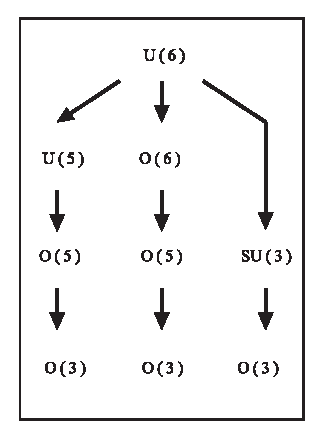
\includegraphics[scale=.65]{img/figure}
	%
	% If not, use
	%\picplace{5cm}{2cm} % Give the correct figure height and width in cm
	%
	\caption{If the width of the figure is less than 7.8 cm use the \texttt{sidecapion} command to flush the caption on the left side of the page. If the figure is positioned at the top of the page, align the sidecaption with the top of the figure -- to achieve this you simply need to use the optional argument \texttt{[t]} with the \texttt{sidecaption} command}
	\label{fig:1}       % Give a unique label
\end{figure}


\paragraph{Paragraph Heading} %
Instead of simply listing headings of different levels we recommend to let every heading be followed by at least a short passage of text. Furtheron please use the \LaTeX\ automatism for all your cross-references and citations as has already been described in Sect.~\ref{sec:2}.

Please note that the first line of text that follows a heading is not indented, whereas the first lines of all subsequent paragraphs are.

For typesetting numbered lists we recommend to use the \verb|enumerate| environment -- it will automatically render Springer's preferred layout.

\begin{enumerate}
	\item{Livelihood and survival mobility are oftentimes coutcomes of uneven socioeconomic development.}
	\begin{enumerate}
		\item{Livelihood and survival mobility are oftentimes coutcomes of uneven socioeconomic development.}
		\item{Livelihood and survival mobility are oftentimes coutcomes of uneven socioeconomic development.}
	\end{enumerate}
	\item{Livelihood and survival mobility are oftentimes coutcomes of uneven socioeconomic development.}
\end{enumerate}


\subparagraph{Subparagraph Heading} In order to avoid simply listing headings of different levels we recommend to let every heading be followed by at least a short passage of text. Use the \LaTeX\ automatism for all your cross-references and citations as has already been described in Sect.~\ref{sec:2}, see also Fig.~\ref{fig:2}.

Please note that the first line of text that follows a heading is not indented, whereas the first lines of all subsequent paragraphs are.

For unnumbered list we recommend to use the \verb|itemize| environment -- it will automatically render Springer's preferred layout.

\begin{itemize}
	\item{Livelihood and survival mobility are oftentimes coutcomes of uneven socioeconomic development, cf. Table~\ref{tab:1}.}
	\begin{itemize}
		\item{Livelihood and survival mobility are oftentimes coutcomes of uneven socioeconomic development.}
		\item{Livelihood and survival mobility are oftentimes coutcomes of uneven socioeconomic development.}
	\end{itemize}
	\item{Livelihood and survival mobility are oftentimes coutcomes of uneven socioeconomic development.}
\end{itemize}

\begin{figure}[t]
	\centering
	% Use the relevant command for your figure-insertion program
	% to insert the figure file.
	% For example, with the option graphics use
	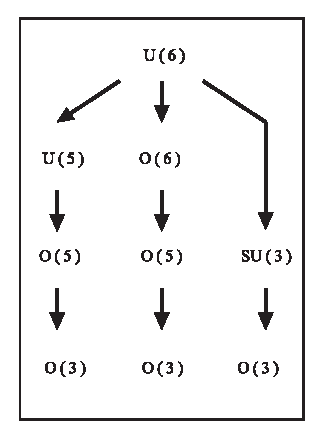
\includegraphics[scale=.65]{img/figure}
	%
	% If not, use
	%\picplace{5cm}{2cm} % Give the correct figure height and width in cm
	%
	\caption{Please write your figure caption here}
	\label{fig:2}       % Give a unique label
\end{figure}

\runinhead{Run-in Heading Boldface Version} Use the \LaTeX\ automatism for all your cross-references and citations as has already been described in Sect.~\ref{sec:2}.

\subruninhead{Run-in Heading Boldface and Italic Version} Use the \LaTeX\ automatism for all your cross-refer\-ences and citations as has already been described in Sect.~\ref{sec:2}\index{paragraph}.

\subsubruninhead{Run-in Heading Displayed Version} Use the \LaTeX\ automatism for all your cross-refer\-ences and citations as has already been described in Sect.~\ref{sec:2}\index{paragraph}.
% Use the \index{} command to code your index words
%
% For tables use
%
\begin{table}[!t]
	\caption{Please write your table caption here}
	\label{tab:1}       % Give a unique label
	%
	% For LaTeX tables use
	%
	\begin{tabular}{p{2cm}p{2.4cm}p{2cm}p{4.9cm}}
		\hline\noalign{\smallskip}
		Classes & Subclass & Length & Action Mechanism  \\
		\noalign{\smallskip}\svhline\noalign{\smallskip}
		Translation & mRNA$^a$  & 22 (19--25) & Translation repression, mRNA cleavage\\
		Translation & mRNA cleavage & 21 & mRNA cleavage\\
		Translation & mRNA  & 21--22 & mRNA cleavage\\
		Translation & mRNA  & 24--26 & Histone and DNA Modification\\
		\noalign{\smallskip}\hline\noalign{\smallskip}
	\end{tabular}
	$^a$ Table foot note (with superscript)
\end{table}
%
\section{Section Heading}\label{sec:1}
\label{sec:3}
% Always give a unique label
% and use \ref{<label>} for cross-references
% and \cite{<label>} for bibliographic references
% use \sectionmark{}
% to alter or adjust the section heading in the running head
Instead of simply listing headings of different levels we recommend to let every heading be followed by at least a short passage of text. Furtheron please use the \LaTeX\ automatism for all your cross-references and citations as has already been described in Sect.~\ref{sec:2}.

Please note that the first line of text that follows a heading is not indented, whereas the first lines of all subsequent paragraphs are.

If you want to list definitions or the like we recommend to use the Springer-enhanced \verb|description| environment -- it will automatically render Springer's preferred layout.

\begin{description}[Type 1]
	\item[Type 1]{That addresses central themes pertainng to migration, health, and disease. In Sect.~\ref{sec:1}, Wilson discusses the role of human migration in infectious disease distributions and patterns.}
	\item[Type 2]{That addresses central themes pertainng to migration, health, and disease. In Sect.~\ref{subsec:2}, Wilson discusses the role of human migration in infectious disease distributions and patterns.}
\end{description}

\subsection{Subsection Heading} \label{sec:2}
In order to avoid simply listing headings of different levels we recommend to let every heading be followed by at least a short passage of text. Use the \LaTeX\ automatism for all your cross-references and citations citations as has already been described in Sect.~\ref{sec:2}.

Please note that the first line of text that follows a heading is not indented, whereas the first lines of all subsequent paragraphs are.

\begin{svgraybox}
	If you want to emphasize complete paragraphs of texts we recommend to use the newly defined Springer class option \verb|graybox| and the newly defined environment \verb|svgraybox|. This will produce a 15 percent screened box 'behind' your text.
	
	If you want to emphasize complete paragraphs of texts we recommend to use the newly defined Springer class option and environment \verb|svgraybox|. This will produce a 15 percent screened box 'behind' your text.
\end{svgraybox}


\subsubsection{Subsubsection Heading}
Instead of simply listing headings of different levels we recommend to let every heading be followed by at least a short passage of text. Furtheron please use the \LaTeX\ automatism for all your cross-references and citations as has already been described in Sect.~\ref{sec:2}.

Please note that the first line of text that follows a heading is not indented, whereas the first lines of all subsequent paragraphs are.

\begin{theorem}
Theorem text goes here.
\end{theorem}
%
% or
%
\begin{definition}
Definition text goes here.
\end{definition}

\begin{proof}
	%\smartqed
	Proof text goes here.
	%\qed
\end{proof}

\paragraph{Paragraph Heading} %
Instead of simply listing headings of different levels we recommend to let every heading be followed by at least a short passage of text. Furtheron please use the \LaTeX\ automatism for all your cross-references and citations as has already been described in Sect.~\ref{sec:2}.

Note that the first line of text that follows a heading is not indented, whereas the first lines of all subsequent paragraphs are.
%
% For built-in environments use
%


\begin{theorem}
	Theorem text goes here.
\end{theorem}
%
\begin{definition}
	Definition text goes here.
\end{definition}
%
\begin{proof}
	%\smartqed
	Proof text goes here.
	%\qed
\end{proof}
%
%
\begin{trailer}{Trailer Head}
	If you want to emphasize complete paragraphs of texts in an \verb|Trailer Head| we recommend to
	use  \begin{verbatim}\begin{trailer}{Trailer Head}
			...
	\end{trailer}\end{verbatim}
\end{trailer}
%
\begin{question}{Kérdések}
	If you want to emphasize complete paragraphs of texts in an \verb|Questions| we recommend to
	use  \begin{verbatim}\begin{question}{Kérdések}
			...
	\end{question}\end{verbatim}
\end{question}
%
%
\begin{important}{Important}
	If you want to emphasize complete paragraphs of texts in an \verb|Important| we recommend to
	use  \begin{verbatim}\begin{important}{Important}
			...
	\end{important}\end{verbatim}
\end{important}

\begin{warning}{Figyelem}
	If you want to emphasize complete paragraphs of texts in an \verb|Attention| we recommend to
	use  \begin{verbatim}\begin{warning}{Figyelem}
			...
	\end{warning}\end{verbatim}
\end{warning}

\begin{programcode}{Programrész}
	If you want to emphasize complete paragraphs of texts in an \verb|Program Code| we recommend to
	use
	
	\verb|\begin{programcode}{Programrész}|
		
		\verb|\begin{verbatim}...\end{verbatim}|
		
		\verb|\end{programcode}|
	
\end{programcode}
%
\begin{tips}{Tippek}
	If you want to emphasize complete paragraphs of texts in an \verb|Tips| we recommend to
	use  \begin{verbatim}\begin{tips}{Tippek}
			...
	\end{tips}\end{verbatim}
\end{tips}
%
%
\begin{overview}{Áttekintés}
	If you want to emphasize complete paragraphs of texts in an \verb|Overview| we recommend to
	use  \begin{verbatim}\begin{overview}{Áttekintés}
			...
	\end{overview}\end{verbatim}
\end{overview}

\begin{backgroundinformation}{Background Information}
	If you want to emphasize complete paragraphs of texts in an \verb|Background|
	\verb|Information| we recommend to
	use
	
	\verb|\begin{backgroundinformation}{Background Information}|
		
		\verb|...|
		
		\verb|\end{backgroundinformation}|
\end{backgroundinformation}
\begin{legaltext}{Legal Text}
	If you want to emphasize complete paragraphs of texts in an \verb|Legal Text| we recommend to
	use  \begin{verbatim}\begin{legaltext}{Legal Text}
			...
	\end{legaltext}\end{verbatim}
\end{legaltext}
%
\begin{acknowledgement}
	If you want to include acknowledgments of assistance and the like at the end of an individual chapter please use the \verb|acknowledgement| environment -- it will automatically render Springer's preferred layout.
\end{acknowledgement}
%

\begin{equation}
	a \times b = c
\end{equation}
% Problems or Exercises should be sorted chapterwise
\section*{Problems}
%
% Use the following environment.
% Don't forget to label each problem;
% the label is needed for the solutions' environment
\begin{prob}
	\label{prob1}
	A given problem or Excercise is described here. The
	problem is described here. The problem is described here.
\end{prob}

\begin{prob}
	\label{prob2}
	\textbf{Problem Heading}\\
	(a) The first part of the problem is described here.\\
	(b) The second part of the problem is described here.
\end{prob}


\section{Section Heading}
\label{sec:A1}
% Always give a unique label
% and use \ref{<label>} for cross-references
% and \cite{<label>} for bibliographic references
% use \sectionmark{}
% to alter or adjust the section heading in the running head
Instead of simply listing headings of different levels we recommend to let every heading be followed by at least a short passage of text. Furtheron please use the \LaTeX\ automatism for all your cross-references and citations.


\subsection{Subsection Heading}
\label{sec:A2}
Instead of simply listing headings of different levels we recommend to let every heading be followed by at least a short passage of text. Furtheron please use the \LaTeX\ automatism for all your cross-references and citations as has already been described in Sect.~\ref{sec:A1}.

For multiline equations we recommend to use the \verb|eqnarray| environment.
\begin{eqnarray}
	\vec{a}\times\vec{b}=\vec{c} \nonumber\\
	\vec{a}\times\vec{b}=\vec{c}
	\label{eq:A01}
\end{eqnarray}

\subsubsection{Subsubsection Heading}
Instead of simply listing headings of different levels we recommend to let every heading be followed by at least a short passage of text. Furtheron please use the \LaTeX\ automatism for all your cross-references and citations as has already been described in Sect.~\ref{sec:A2}.

Please note that the first line of text that follows a heading is not indented, whereas the first lines of all subsequent paragraphs are.

% For figures use
%
\begin{figure}[t]
	\sidecaption[t]
	%\centering
	% Use the relevant command for your figure-insertion program
	% to insert the figure file.
	% For example, with the option graphics use
	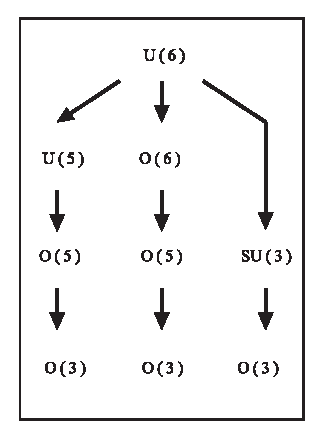
\includegraphics[scale=.65]{img/figure}
	%
	% If not, use
	%\picplace{5cm}{2cm} % Give the correct figure height and width in cm
	%
	\caption{Please write your figure caption here}
	\label{fig:A1}       % Give a unique label
\end{figure}

% For tables use
%
\begin{table}
	\caption{Please write your table caption here}
	\label{tab:A1}       % Give a unique label
	%
	% For LaTeX tables use
	%
	\begin{tabular}{p{2cm}p{2.4cm}p{2cm}p{4.9cm}}
		\hline\noalign{\smallskip}
		Classes & Subclass & Length & Action Mechanism  \\
		\noalign{\smallskip}\hline\noalign{\smallskip}
		Translation & mRNA$^a$  & 22 (19--25) & Translation repression, mRNA cleavage\\
		Translation & mRNA cleavage & 21 & mRNA cleavage\\
		Translation & mRNA  & 21--22 & mRNA cleavage\\
		Translation & mRNA  & 24--26 & Histone and DNA Modification\\
		\noalign{\smallskip}\hline\noalign{\smallskip}
	\end{tabular}
	$^a$ Table foot note (with superscript)
\end{table}
%

Examples for references: \cite{PlatypOUsGIT}, \cite{angeles2002fundamentals}, \cite{householder1964theory}, \cite{RozsaPalMatrix}

\newpage
\bibliographystyle{IEEEtran}
\bibliography{refs}
	

\end{document}





